% !TEX root = Master.tex

This study faces several major challenges which need to be resolved in the analysis:

\renewcommand{\labelenumi}{\arabic{enumi}.}
\begin{enumerate}

\item As mentioned, the tree detection algorithm based on LiDAR imposes a systematic bias.
Subdominant trees which are covered by dominant tree crowns cannot be detected (see Figure \ref{fig:dominant_trees}).
Unfortunately, the height of the covered trees cannot be determined. This leads to a systematic overestimation of the tree diameter distribution of each compartment. The covered tree height cannot be determined but must be within the interval 5m < x < height of covering tree. The main task of this study is to correct for this bias.

\item Although the diameter of over 10000 trees are collected, only 23 compartments have 40 or more
measured trees. This problem is aggravated as \textasciitilde 700 of the 1642 compartments don’t have any measurements.
Meaning that a distribution fitting via Maximum Likelihood Estimation for compartments with too little or no data must be performed.

\item The measured data for the regression is unreliable. Tree species, crown area and height are
detected by LiDAR for the inventory dataset. Whereby the tree species is detected by neural networks with an approximate 85\% accuracy. The tree diameter differs depending on the species significantly (as seen in Section \ref{Regression Models}), which results in additional bias in the prediction.

\item The fourth challenge was discovered in Section \ref{Clustering}. Dominant (large) trees cannot only
cover subdominant (smaller) trees, but equally tall trees might be detected as only one tree (see Figure \ref{fig:dominant_trees}). As a result, the crown area will be significantly overestimated in the inventory dataset which is used in the regression resulting in addtional bias in the prediction.

\begin{figure}[H]
  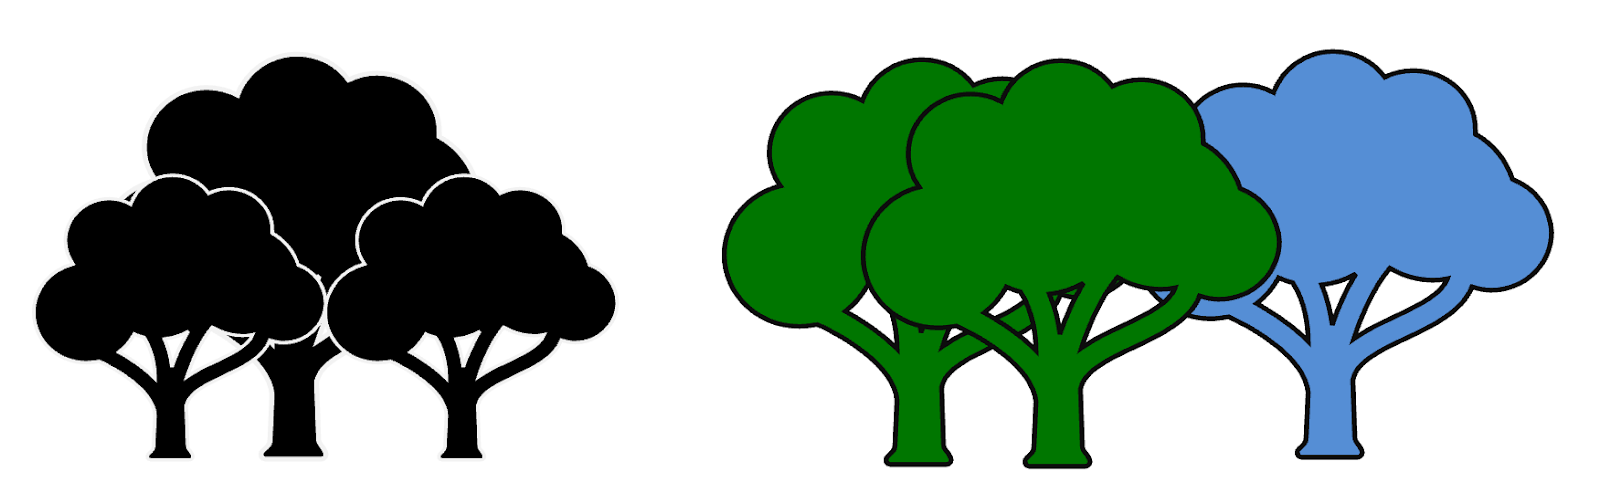
\includegraphics[width=\textwidth]{dominant_trees.png}
  \caption{Visualization of detection problems.\\ Left: a dominant tree covers subdominant
trees (challange 1).\\ Right: Close equally tall trees (green) are detected as one tree, causing
overestimation of the crown area (challange 4).}
  \label{fig:dominant_trees}
\end{figure}

\end{enumerate}